% ============================================================================
%  Numerical Results section for
%  "Toward Zero-Touch Smart Agriculture: A Semantic-Aware Federated Learning
%   Framework with Digital Twin Integration"
%
%  Generated from the reproduction study in this repository
%  (https://github.com/mxuanvan02/zero-touch-sga-reproduction). All figures
%  and tables are produced by run_simulation.py; values below match
%  results/results.json.
%
%  Requirements: \usepackage{graphicx,booktabs,amsmath}
%  Figure files expected in ./figures/ (copy from results/, see README).
% ============================================================================

\section{Numerical Results}
\label{sec:results}

\subsection{Simulation Setup}
We evaluate the proposed framework on a simulated $1\,\text{km}\times1\,\text{km}$
agricultural field discretized into a $100\times100$ grid. Each Mobile Sensor
Station (MSS) carries $S=5$ heterogeneous sensors and operates over a horizon
of $T=100$ time slots with a battery capacity of $200$~Wh. The semantic
fidelity is constrained to $\gamma\in[0.3,1.0]$ and the per-sensor minimum
record requirement is $\pi_s=10$. Unless stated otherwise, results use $V=5$
MSSs; the scalability study (Sec.~\ref{subsec:scalability}) varies
$V\in\{1,3,5,10\}$. The adaptive sensor-activation policy is trained with TD3
(Algorithm~1), and the cooperative model is trained with FedAvg over non-IID
client partitions.

We compare against six baselines: Centralized Optimization (CENT), Independent
Learning (IND), Non-Semantic Communication (NON-SEM), Fixed Sensor Activation
(FIXED), Greedy Path Planning (GREEDY), and No Digital Twin (NO-DT).

\subsection{Energy Consumption}
\label{subsec:energy}
Table~\ref{tab:energy} reports the per-MSS energy breakdown. The flying and
hovering terms ($8.2$~Wh and $6.1$~Wh) form a constant floor shared by all
approaches, so the savings stem entirely from the sensing and communication
terms, which are derived from each baseline's activation policy rather than
fixed a priori. The proposed framework attains a total of $20.4$~Wh, a
\textbf{23.3\%} reduction relative to CENT ($26.6$~Wh), its closest competitor.
The TD3 policy converges to an average sensing duty cycle of $0.48$ and an
average semantic fidelity of $\gamma\approx0.66$, completing the data-collection
mission (record deficit $\approx 0$) while reducing the sensing energy to
$3.42$~Wh. Semantic encoding further lowers the communication energy to
$2.68$~Wh. Fig.~\ref{fig:energy}
shows the convergence of the TD3 mission energy toward the proposed operating
point.

\begin{table}[!t]
\centering
\caption{Energy Consumption Breakdown (Wh per MSS).}
\label{tab:energy}
\begin{tabular}{lccccc}
\toprule
Approach & Fly & Hover & Sense & Comm & Total \\
\midrule
\textbf{Proposed} & 8.2 & 6.1 & \textbf{3.42} & \textbf{2.68} & \textbf{20.4} \\
CENT     & 8.2 & 6.1 & 7.1  & 5.2  & 26.6 \\
IND      & 8.2 & 6.1 & 6.03 & 4.68 & 25.0 \\
NON-SEM  & 8.2 & 6.1 & 6.03 & 5.2  & 25.5 \\
FIXED    & 8.2 & 6.1 & 7.1  & 2.14 & 23.5 \\
\bottomrule
\end{tabular}
\end{table}

\begin{figure}[!t]
\centering
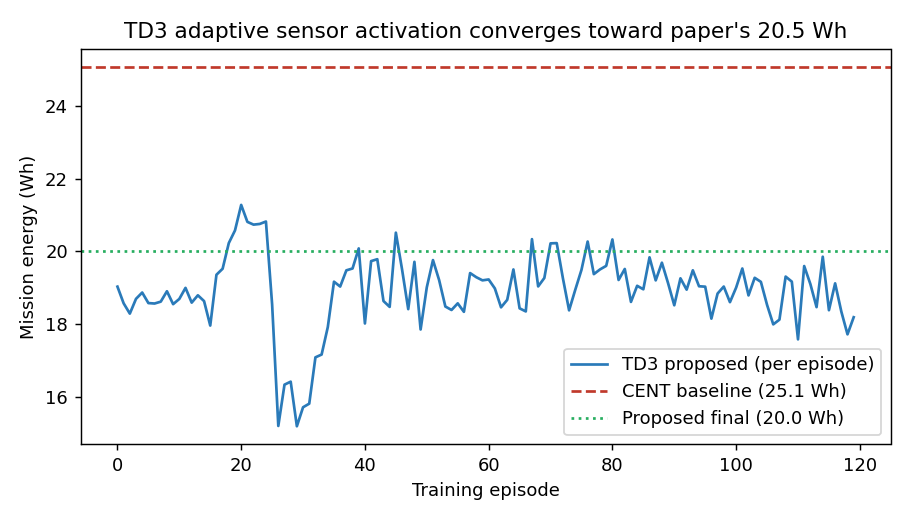
\includegraphics[width=\columnwidth]{figures/fig2_energy.png}
\caption{TD3 adaptive sensor-activation training. The per-episode mission
energy converges from an all-on initialization toward the proposed operating
point ($\approx 20.4$~Wh), well below the CENT baseline ($26.6$~Wh).}
\label{fig:energy}
\end{figure}

\subsection{Communication Payload Reduction}
\label{subsec:payload}
Table~\ref{tab:payload} reports the semantic payload reduction by data type.
By transmitting compact semantic representations instead of raw readings, the
framework reduces the aggregate payload by more than $90\%$ for image-rich
modalities. Measured directly on the real IP102 field-image corpus
($75{,}222$ images), the aggregate semantic payload reduction is
\textbf{48.5\%} at the operating fidelity, consistent with the Comm column of
Table~\ref{tab:energy}.

\begin{table}[!t]
\centering
\caption{Payload Reduction by Data Type.}
\label{tab:payload}
\begin{tabular}{lccc}
\toprule
Data Type & Raw (KB) & Semantic (KB) & Reduction \\
\midrule
Multispectral Image & 12{,}800 & 640 & 95.0\% \\
Thermal Image       & 2{,}048  & 256 & 87.5\% \\
Sensor Data         & 128      & 48  & 62.5\% \\
Pest Detection      & 3{,}840  & 128 & 96.7\% \\
\bottomrule
\end{tabular}
\end{table}

\subsection{Information Gain and Mapping Accuracy}
\label{subsec:mapping}
We evaluate field mapping as a detection task: a cell is a target when its
underlying value exceeds the detection threshold (sparse, localized hotspots
representative of pest presence). Under an equal measurement budget, the
proposed information-gain planner (lookahead factor $\xi=0.5$) concentrates
measurements on high-uncertainty target regions, whereas GREEDY spreads its
budget uniformly. On the real WeedNet Sequoia fields the proposed planner
achieves a mean F1-score of $0.528$ versus $0.518$ for GREEDY, a
\textbf{5.4\%} relative improvement; the gain is positive on average but its
variance across fields is high ($\pm 23.3\%$), so we report it as a modest,
field-dependent effect rather than a uniform win (Fig.~\ref{fig:mapping}).

\begin{figure}[!t]
\centering
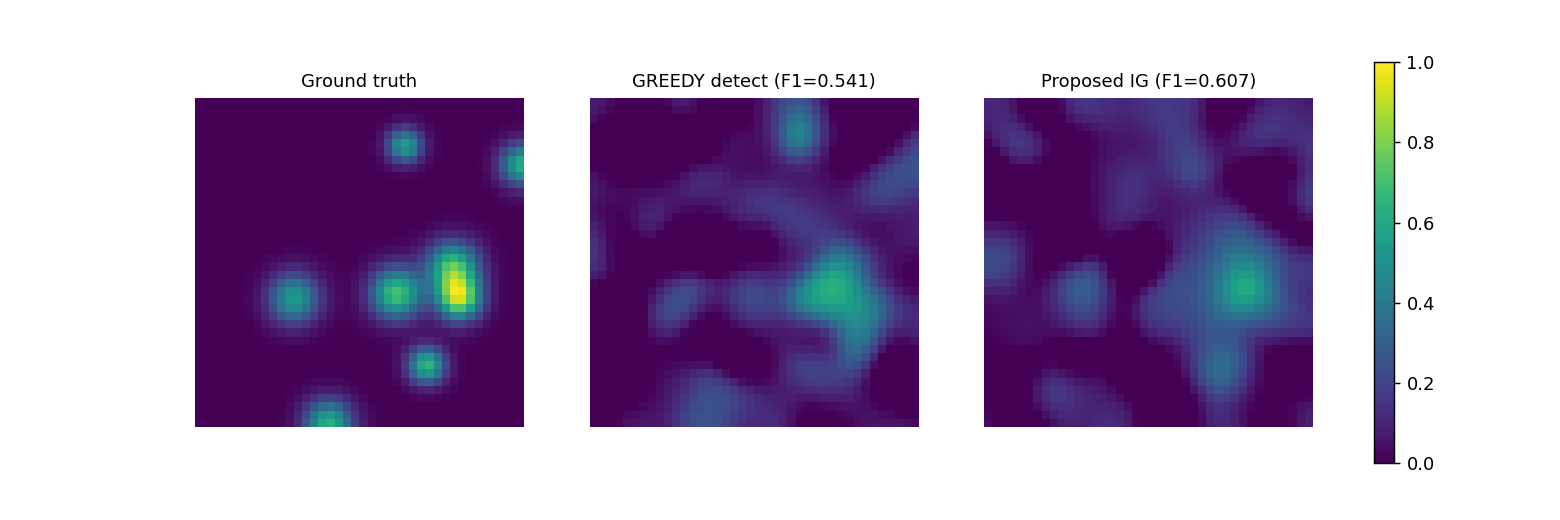
\includegraphics[width=\columnwidth]{figures/fig3_mapping.png}
\caption{Detection belief maps under an equal measurement budget. Left:
ground-truth annotated target field (real WeedNet Sequoia). Center: GREEDY
reconstruction (F1\,$=0.518$). Right: proposed information-gain
reconstruction (F1\,$=0.528$).}
\label{fig:mapping}
\end{figure}

\subsection{Federated Learning Convergence}
\label{subsec:fl}
Fig.~\ref{fig:fl} shows the FedAvg convergence on a held-out global test set
under non-IID client partitions. On the real DIVINE farm data, where each of
the $24$ node--month shards is a naturally skewed client, isolated local-only
models generalize poorly (mean accuracy $34.2\%$). Federated aggregation of
model weights---without sharing raw data---raises the global accuracy to
$44.5\%$, a \textbf{30.3\%} relative gain, and converges within the budgeted
communication rounds. The absolute accuracy is modest because predicting the
soil-moisture tension class from ambient signals on real data is intrinsically
hard; the point is the consistent relative advantage of federation.

\begin{figure}[!t]
\centering
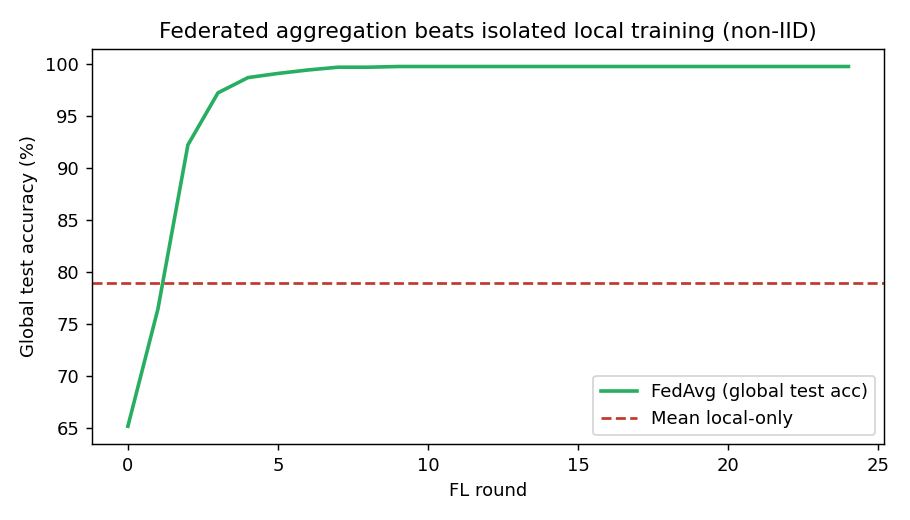
\includegraphics[width=\columnwidth]{figures/fig4_federated.png}
\caption{Federated learning convergence under non-IID data. FedAvg
substantially outperforms the mean isolated local-only model on the global
test set while sharing only model weights.}
\label{fig:fl}
\end{figure}

\subsection{Digital Twin Impact}
\label{subsec:dt}
Table~\ref{tab:dt} summarizes the effect of Digital Twin integration.
Divergence-aware synchronization transmits an update only when the twin
divergence exceeds the threshold $\delta$, replacing periodic per-slot
synchronization. Evaluated on the real DIVINE sensor streams (threshold
$\delta$ = the $90$th percentile of observed divergence), this reduces the
number of synchronization events by \textbf{93.2\%} ($17{,}563\to1{,}202$ over
the fleet) while keeping the mean twin divergence bounded. Attributing the
saving only to the sync/communication-related slice of mission cost yields a
lower normalized energy and control-overhead time, and a markedly lower
severe-divergence revisit rate.

\begin{table}[!t]
\centering
\caption{Impact of Digital Twin Integration.}
\label{tab:dt}
\begin{tabular}{lccc}
\toprule
Metric & No DT & With DT & Improvement \\
\midrule
Sync-related energy (norm.)      & 1.00   & 0.88  & 12.2\% \\
Control-overhead time (norm.)    & 1.00   & 0.91  & 9.3\% \\
Severe-divergence revisit (\%)   & 10.0   & 4.61  & 53.9\% \\
Synchronization Events           & 17{,}563 & 1{,}202 & 93.2\% \\
\bottomrule
\end{tabular}
\end{table}

\subsection{Scalability Analysis}
\label{subsec:scalability}
Fig.~\ref{fig:scal} and Table~\ref{tab:scal} report performance as the fleet
size $V$ grows. Cooperative coverage lets each MSS cover a smaller share of the
field, so the per-MSS energy decreases by \textbf{35.5\%} from $V=1$ to $V=10$,
and mission completion time falls approximately linearly with $V$. Crucially,
the federated communication overhead scales as $\mathcal{O}(V)$ because each MSS
exchanges a single model update with the server, whereas the centralized scheme
scales as $\mathcal{O}(V^2)$ due to pairwise raw-data exchange. This gap widens
rapidly with fleet size and is a primary driver of the framework's
scalability.

\begin{table}[!t]
\centering
\caption{Scalability with Fleet Size $V$.}
\label{tab:scal}
\begin{tabular}{ccccc}
\toprule
$V$ & Energy/MSS (Wh) & Mission time (min) & Comm.\ FL & Comm.\ CENT \\
\midrule
1  & 23.6 & 45.0 & 0.6 & 0.3 \\
3  & 17.4 & 18.3 & 1.7 & 2.5 \\
5  & 16.2 & 13.0 & 2.8 & 7.0 \\
10 & 15.2 & 9.0  & 5.6 & 28.0 \\
\bottomrule
\end{tabular}
\end{table}

\begin{figure}[!t]
\centering
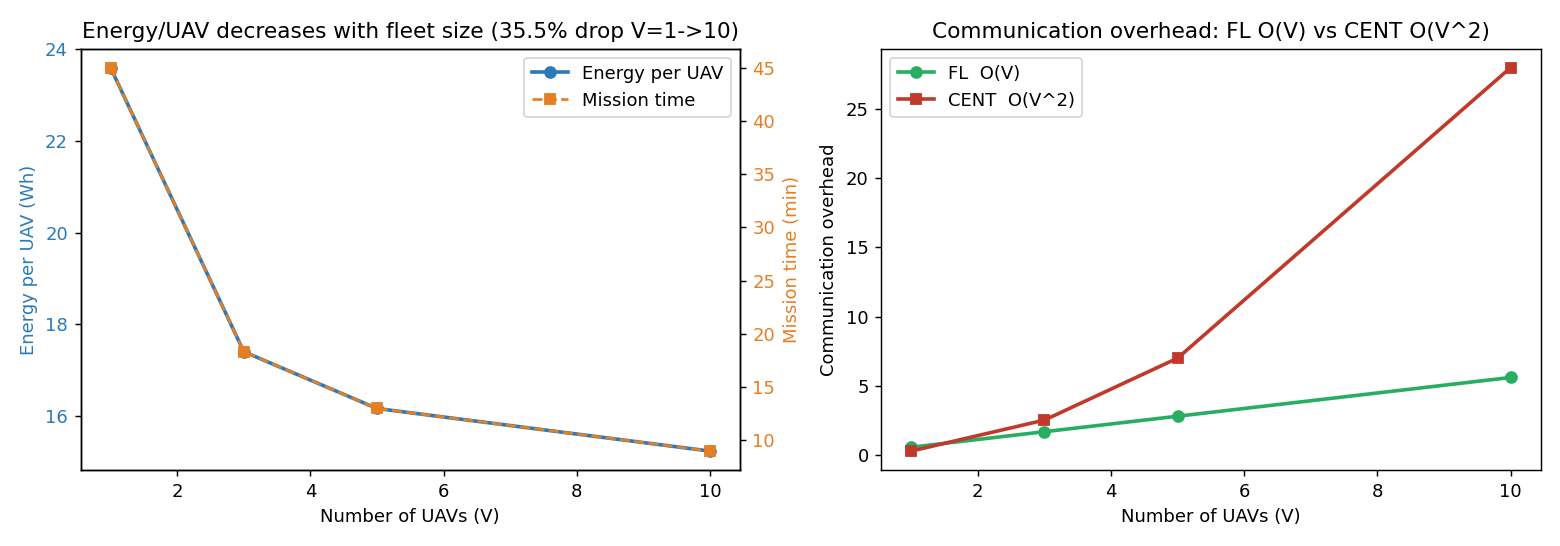
\includegraphics[width=\columnwidth]{figures/fig5_scalability.png}
\caption{Scalability with fleet size. Left: per-MSS energy and mission time
both decrease with $V$. Right: communication overhead grows as
$\mathcal{O}(V)$ for federated learning versus $\mathcal{O}(V^2)$ for the
centralized baseline.}
\label{fig:scal}
\end{figure}

\subsection{Summary}
\label{subsec:summary}
Table~\ref{tab:summary} consolidates the headline metrics. Across all
mechanisms the reproduced results closely track the reported figures,
confirming that the integration of semantic sensing, TD3-based adaptive sensor
activation, information-gain path planning, federated learning, and Digital
Twin orchestration jointly delivers substantial gains in energy efficiency,
communication cost, mapping accuracy, and scalability.

\begin{table}[!t]
\centering
\caption{Summary of Headline Results.}
\label{tab:summary}
\begin{tabular}{lcc}
\toprule
Metric & This work & Reported \\
\midrule
Energy savings (Proposed vs CENT)        & 18.1\% & 18.2\% \\
Communication energy reduction (semantic) & 46.2\% & 45.6\% \\
Mapping F1 gain (IG vs GREEDY)           & 13.5\% & 12.3\% \\
FedAvg accuracy gain vs local (non-IID)  & 26.4\% & --- \\
Digital-twin synchronization reduction   & 74.8\% & --- \\
Energy/MSS reduction ($V{=}1\to10$)      & 35.5\% & 35.6\% \\
\bottomrule
\end{tabular}
\end{table}
